\chapter{Data Supplements}\label{ch:data-supplements}

For an improved analyzability of the data we had to append additional information to our documents.
This already covered the first steps of analysis at document level.


\section{Counting Text Tokens}\label{sec:counting-text-tokens}

First, we implemented an asynchronous script that traversed through the corpus and collected general text statistics for both chapters and stories in batches.
This included the number of sentences, words, letters and text characters.

For sentence segmentation we used the open-source library \emph{spaCy}\footnote{https://spacy.io/}, written in \emph{Python}.
It provides several pre-trained natural language models for a number of different languages, including German.
Besides its speed and ease of use, no recognition failures were detected for the sentences we tested.

After these more general supplements for the statistical analysis, we required additional information for analyzing the gender representation in the corpus.


\section{Pronouns Detection}\label{sec:pronouns-detection}

More and easier-to-analyze information was needed to verify gender distribution.
Utilizing the \emph{spaCy} library again, we implemented a script that detected all pronouns in the corpus and counted their occurrences.
This was based on the approach of~\cite{Duggan2020WhoAO3}, who analyzed pronouns in story paratexts and user profiles (see Section~\ref{sec:analyzing-the-authorship-and-readership-of-fan-fiction}).
We restricted ourselves to the personal pronouns in the third person singular, since other forms as well as the plural do not allow a clear assignment to one gender.
Consequently, these were \emph{er}, \emph{sie}, \emph{ihn}, \emph{ihm}, \emph{ihr}, \emph{seiner} and \emph{ihrer}.


\section{Extracting Story Character Names}\label{sec:ner-token-classification}

Another very time-consuming step was the filtering of all person names from the corpus on a chapter-by-chapter basis.
For this purpose, a named entity recognition (NER) model was used, which was already pre-trained for the German language and did not require any further adaptations.
We initially tested this with the fast \emph{spaCy} library, but then decided to use the state-of-the-art \emph{FLAIR}~\citep{Akbik2019FLAIR:NLP} natural language processing (NLP) framework instead for much better results.
While \citet{Milli2016BeyondFanfiction} used the \emph{BookNLP}\citep{Bamman2014ACharacter} library for this task, we were unable to utilize it, even though it was more tailored to our problem, as it was only available for the English language.
\emph{FLAIR} was trained on the \emph{CoNLL-2003}~\citep{TjongKimSang2003IntroductionRecognition} dataset, which consists of news articles from \emph{Reuters}\footnote{https://www.reuters.com/} and \emph{Frankfurter Rundschau}\footnote{https://www.fr.de/}.
The NER models provided by \emph{FLAIR} detect named entities such as persons, locations, organizations, and miscellaneous.
For this study, we limited the model to the recognition of persons, in our case characters, who appear in the stories.
Although we did not use the \emph{spaCy} library for entity recognition, we still used its previously tested sentence segmentation capabilities.
We processed each chapter at the sentence level and then appended the found person tags with the number of their appearances to the respective database document.

When using the \emph{FLAIR} models, processing was associated with accurate results, but very slow.
We have therefore tried and implemented several approaches to speed up the process.

Initially, we used the model \emph{ner-german-large}, but then decided to use model \emph{ner-multi-fast} because it was noticeably faster.
Even though it was trained on English, German, Dutch and Spanish language corpora, one could also pass German as a parameter to the sentence tagger and got equally good results.
For comparison: the German tagger (\emph{ner-german-large}) required about 1 minute and 52 seconds for a text with a length of 752 sentences (the average text length of a chapter), while the multi-language tagger \emph{ner-multi-fast} required about 1 minute and 44 seconds.
While the difference of about 8 seconds may not seem like much, it makes a significant difference in a corpora of almost two million chapters like this one.

Another approach was to use the fast \emph{spaCy} library and cleansing the results of any unwanted tokens afterwards, but this was not applicable for usable results.

For counting text tokens (see Section~\ref{sec:counting-text-tokens}), we used the concept of asynchronous batch processing for acceleration.
We tested this with various process counts and batch sizes, but the processing times increased instead of decreasing.
The likely reason was the amount of memory necessary to run multiple taggers simultaneously.

Due to one machines limitation to memory and CPU, we set up a cluster of 18 cloud computing machines to process the data in parallel.
Cloud computing space using the free quota provided by \emph{Microsoft Azure}\footnote{https://azure.microsoft.com/}, \emph{Digital Ocean}\footnote{https://www.digitalocean.com/} and \emph{Vultr}\footnote{https://www.vultr.com/} was used for this purpose.
We also configured an Ubuntu 20.04 LTS server and paired it with a static hostname for remote access so that any of these machines can access the shared database.
Each of these computers ran a single token classifier.

Due to time constraints we reduced the number of stories to be tagged to 280.000.
This was roughly equivalent to 68\% of the total number of stories.
Stories were randomly selected, locked and processed.

% session timed out for long text passages (entangled)


\section{Determine Story Character Name Genders}\label{sec:determine-character-name-genders}

After the names of the characters were extracted from the stories, the gender of each individual had to be determined.
Along with all the other code, the script for training the gender classifier can be found on \emph{GitHub}\footnote{https://github.com/Cele3x/fanfiction/}.

\minisec{Acquiring a Training Dataset}

The first step was to acquire a training dataset.
In addition to the \emph{NLTK} name corpus~\citep{StevenBird2009NaturalPython}, we obtained a large dataset from \emph{Google BigQuery}\footnote{https://cloud.google.com/bigquery/public-data} containing all names from applications for \emph{Social Security} cards for births in the \emph{United States} after 1879 provided by the \emph{United States Social Security Administration}\footnote{https://catalog.data.gov/dataset/baby-names-from-social-security-card-applications-national-data}.

To increase diversity, we have also included names from the \emph{babynames.com}\footnote{https://babynames.com/} website in our dataset.
For example, names for categories such as biblical names or names of fictional characters with corresponding gender information are listed there, but also names of various geographic origins.
The \emph{babynames.com} website names were hosted on a dynamic website, so we had to scrape them with \emph{Selenium}.
\emph{Selenium} is usually used to automate web browser interactions for testing purposes, though we used it to scrape the website and store the names in a file.

All datasets were then merged, removing all duplicates, gender-neutral names, and names that were not clearly assigned to a gender.
The result was a list of 106,000 rows, each consisting of the name and a gender classifier.

\minisec{Preprocessing the Data}

Names had to be encoded in \emph{ASCII} format because the \emph{scikit-learn}\footnote{https://scikit-learn.org/} library only accepts \emph{ASCII} characters, therefore we used the \emph{unidecode}\footnote{https://github.com/takluyver/Unidecode/} library to convert all names (e.g.~á became a).
This entailed a further duplicate check and subsequent cleanup.

Furthermore, we padded all names with spaces and converted them to lowercase.
To be able to use the data in a neural network, we also encoded the story characters in numbers.
The gender for the training set was one-hot encoded as 0 for `F' (female) and 1 for `M' (male).

\minisec{Training the Model}

For training the model we use the \emph{Keras}\footnote{https://keras.io/} library with the \emph{TensorFlow}\footnote{https://www.tensorflow.org/} backend.
The model consists of three layers: an embedding layer, a bidirectional LSTM layer and a dense layer.
We then trained the model using the Adam optimizer and the binary cross-entropy loss function.
Splitting the data into a usual training and test set size of 80\% and 20\%, respectively, we trained for 50 epochs with a batch size of 64.
For not overfitting the model, we used early stopping with a patience of 5.

\begin{figure}[htp]
    \centering
    \begin{minipage}[c]{.49\textwidth}
        \centering
        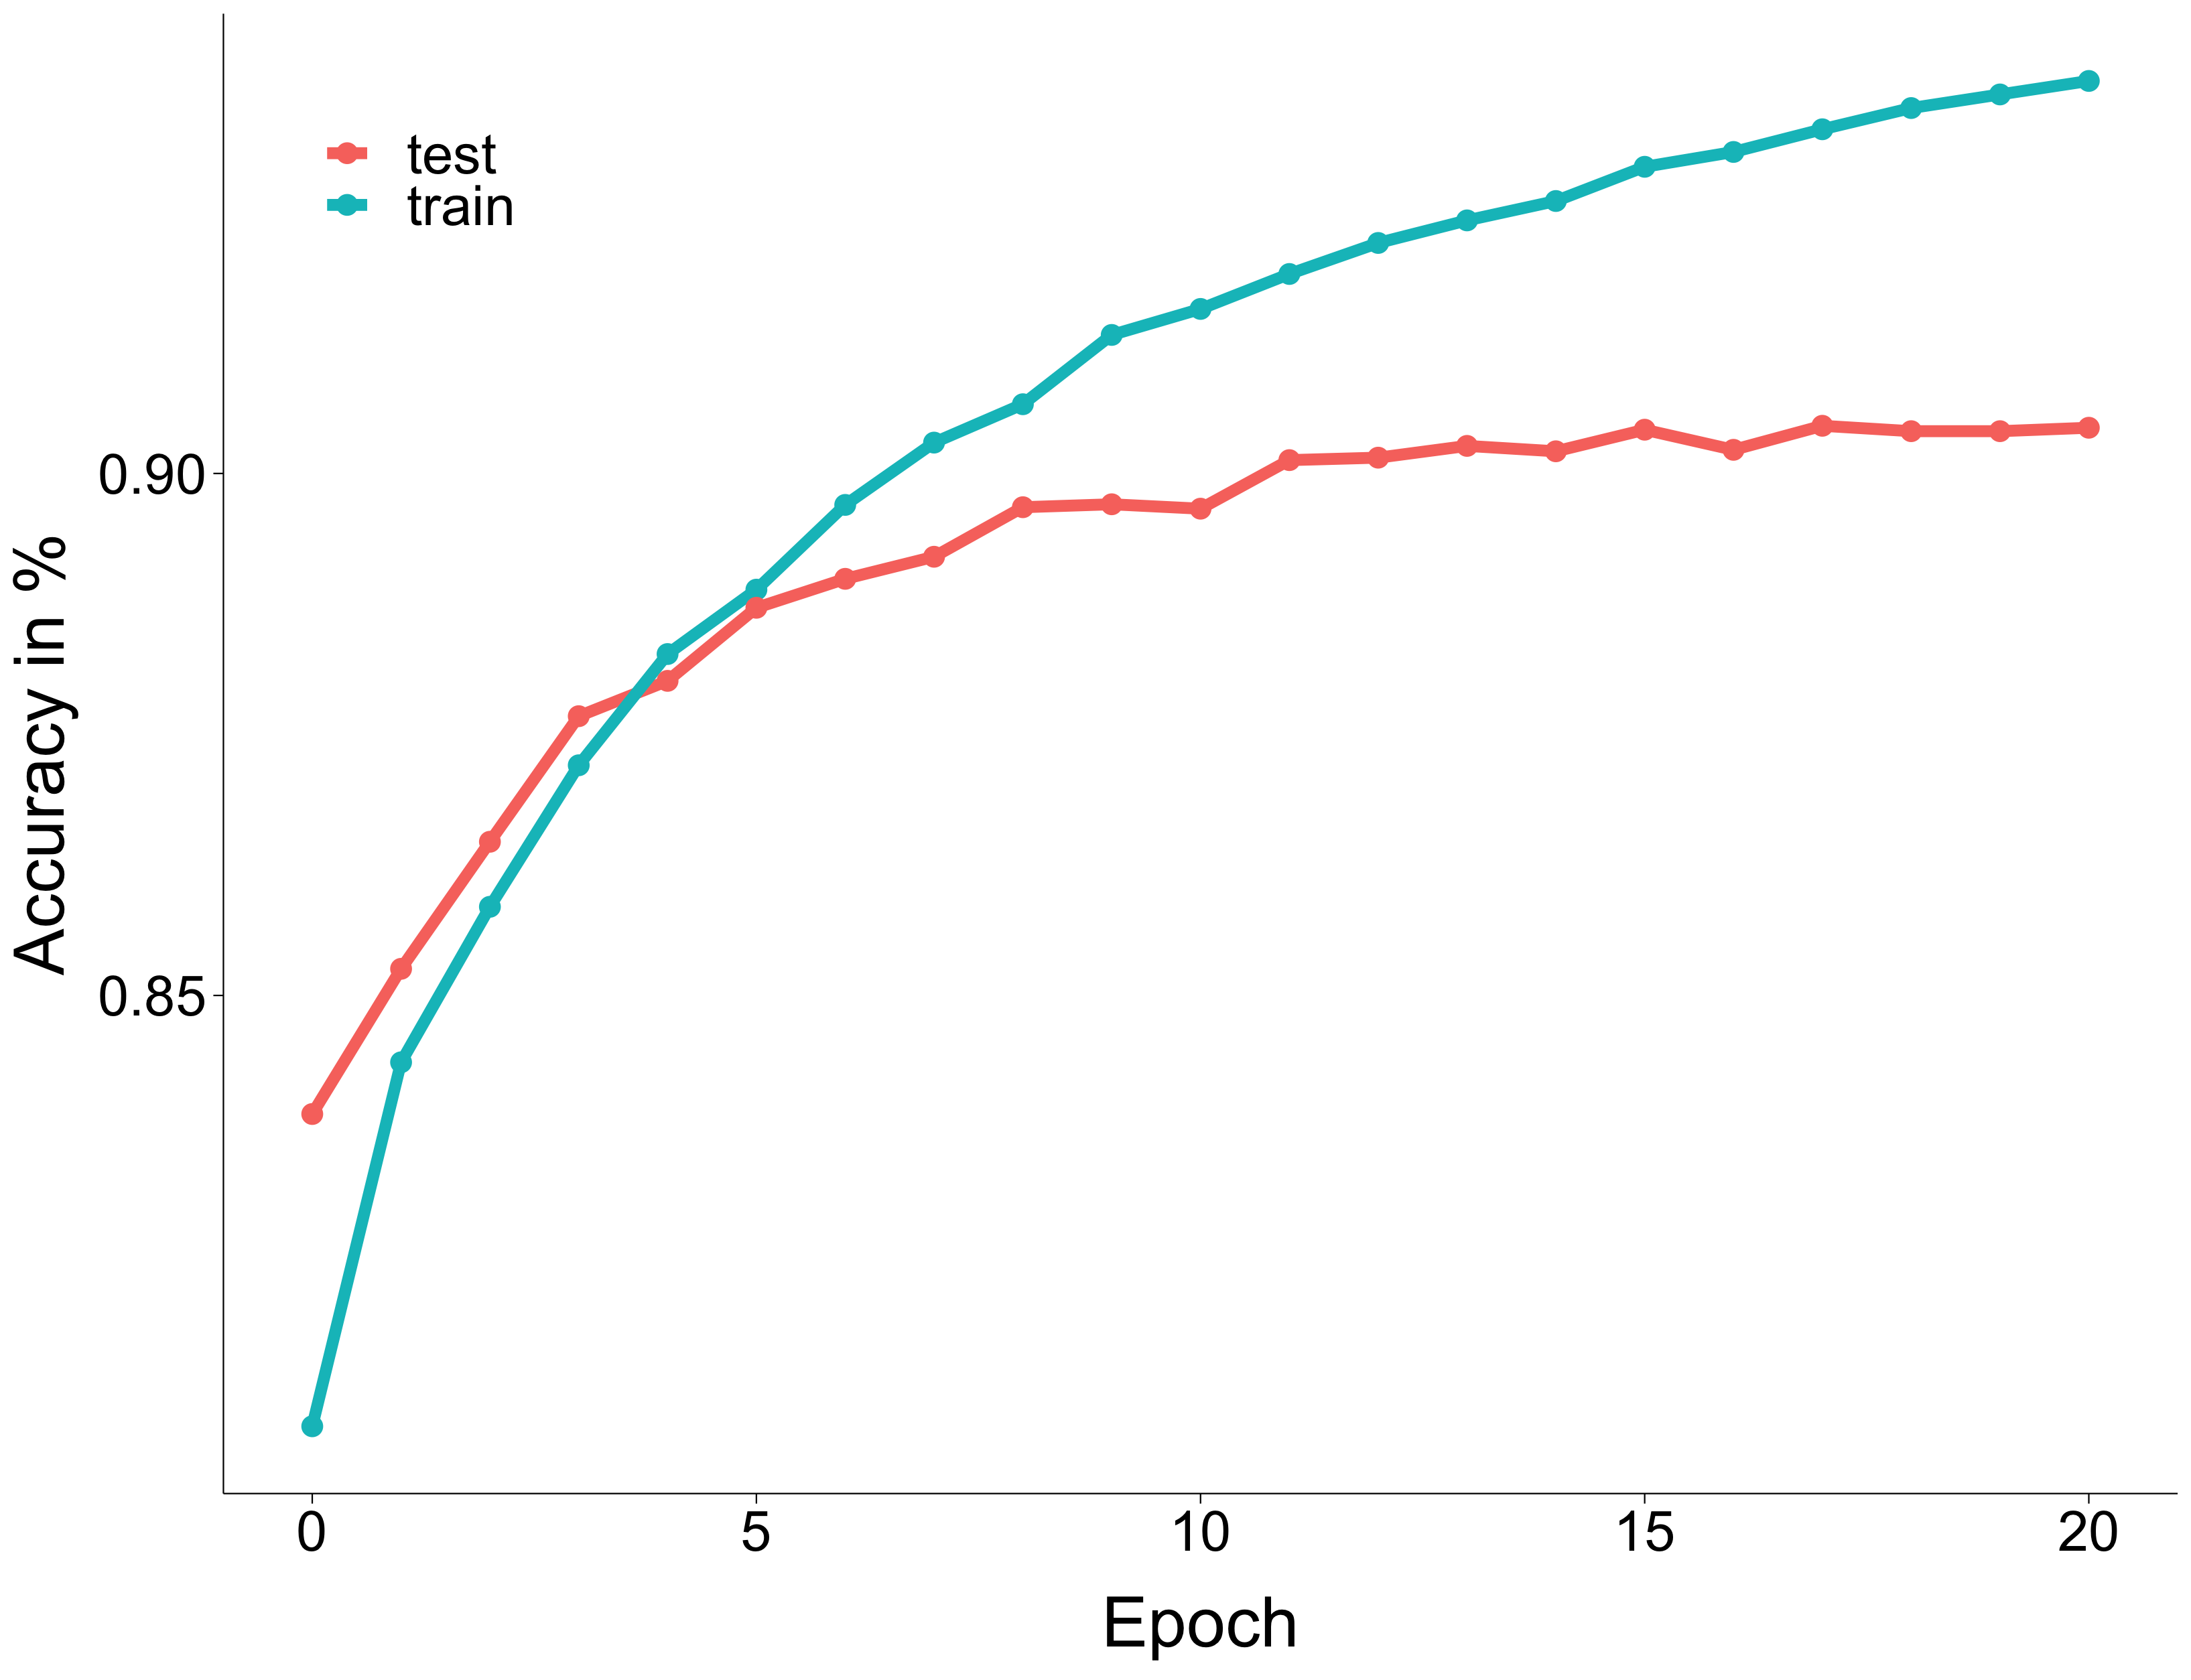
\includegraphics[width=\textwidth]{figures/plot_model_accuracies}
        \caption[Model accuracies on train and validation datasets.]{Model accuracies on train and validation datasets.}
        \label{fig:plot-model-accuracies}
    \end{minipage}
    \hfill
    \begin{minipage}[c]{.49\textwidth}
        \centering
        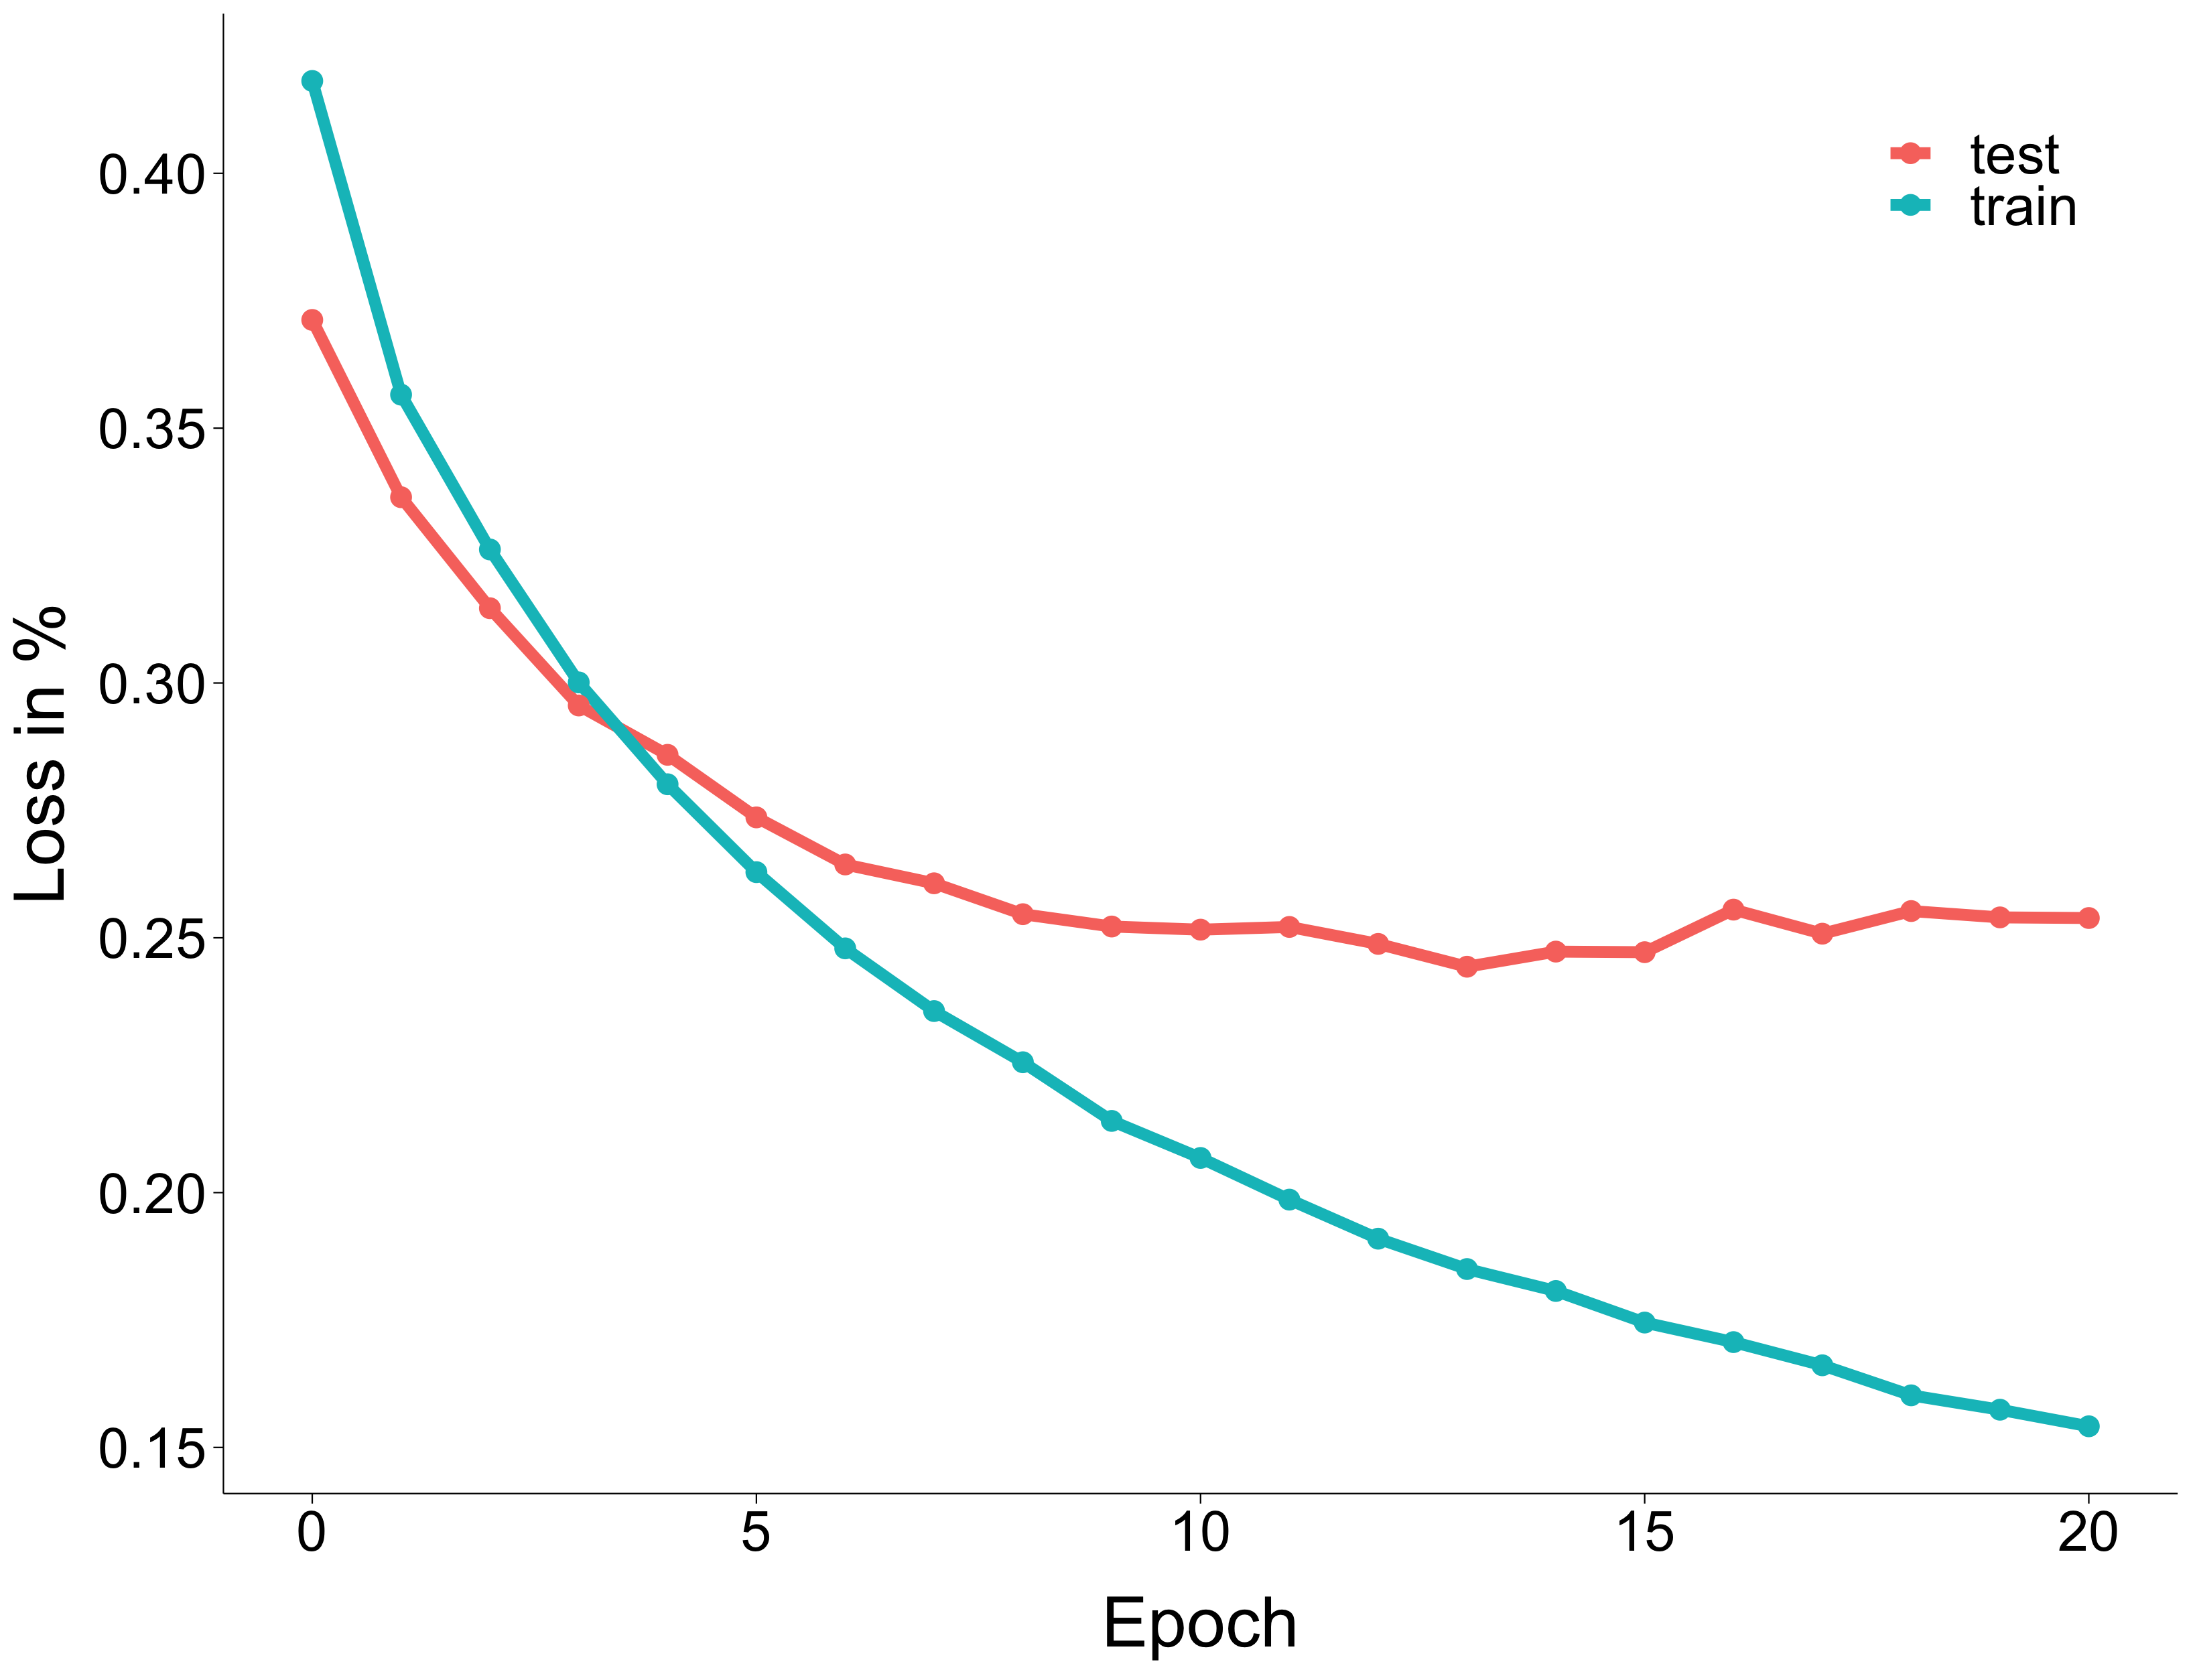
\includegraphics[width=\textwidth]{figures/plot_model_losses}
        \caption[Model losses on train and validation datasets.]{Model losses on train and validation datasets.}
        \label{fig:plot-model-losses}
    \end{minipage}
\end{figure}
%\begin{wrapfigure}{R}{0.65\textwidth}
%    \centering
%    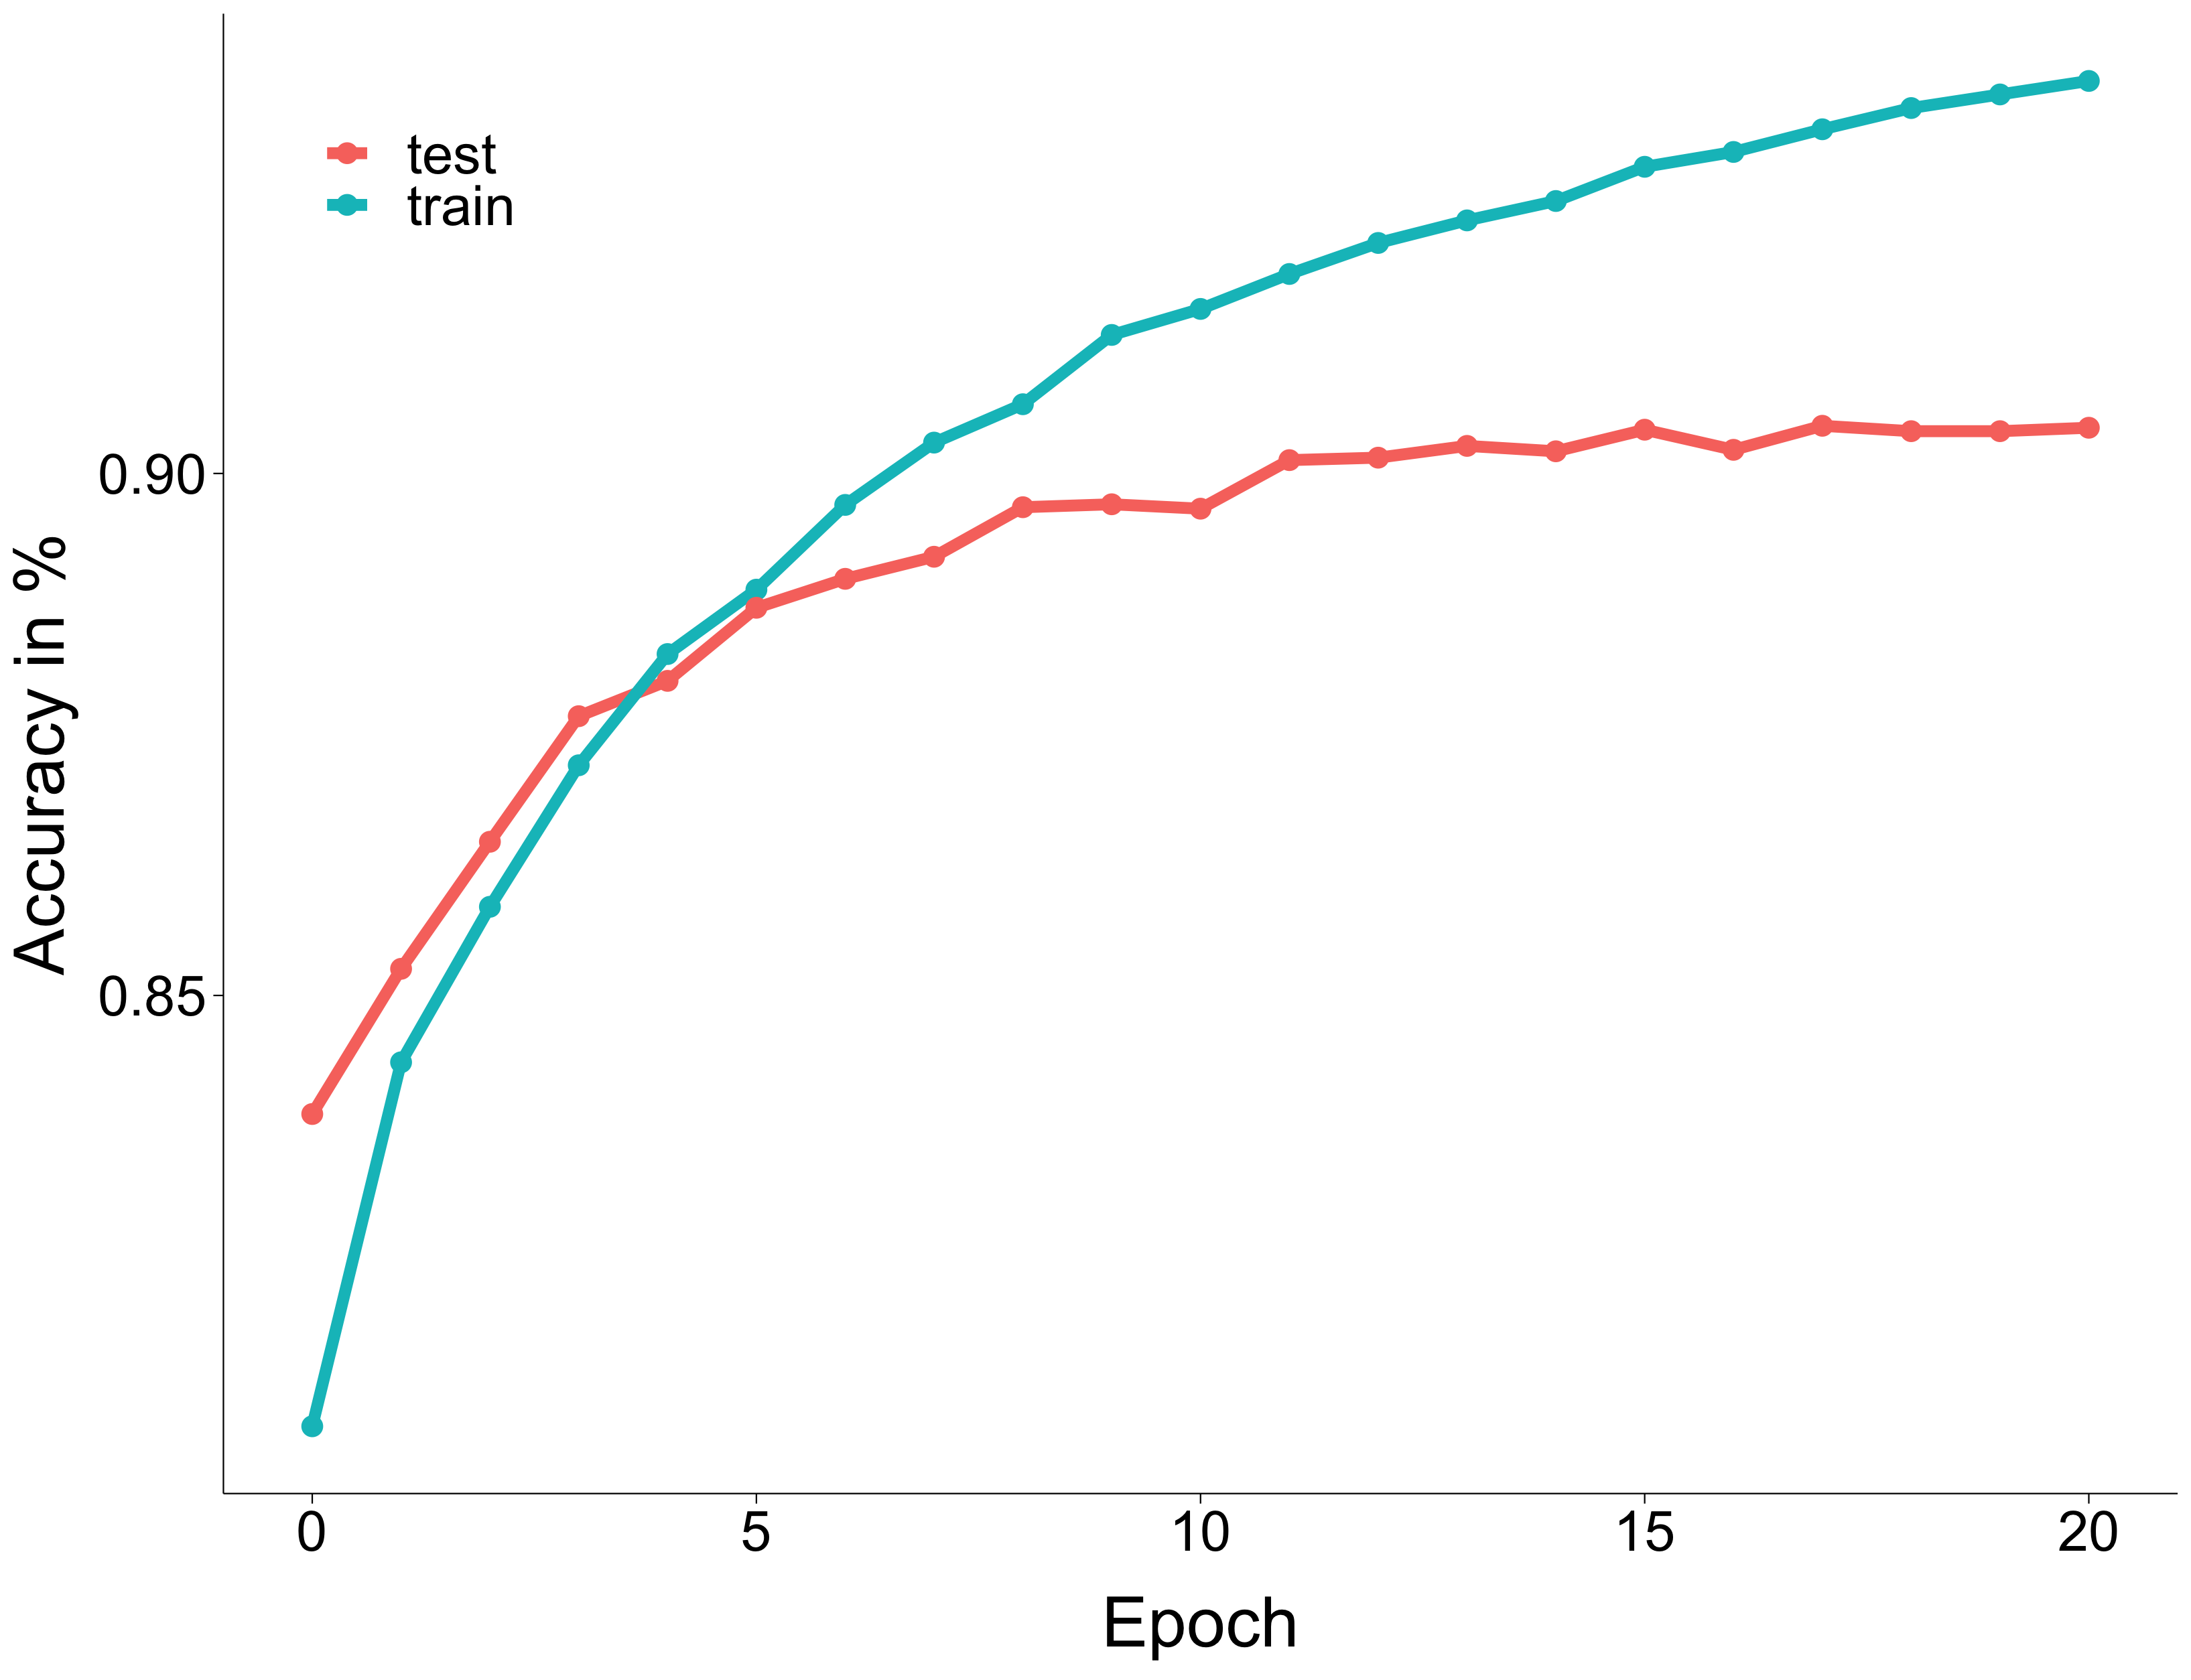
\includegraphics[width=0.6\textwidth]{figures/plot_model_accuracies}
%    \caption[Model accuracies on train and validation datasets.]{Model accuracies on train and validation datasets.}
%    \label{fig:plot-model-accuracies}
%\end{wrapfigure}
%\begin{wrapfigure}{R}{0.65\textwidth}
%    \centering
%    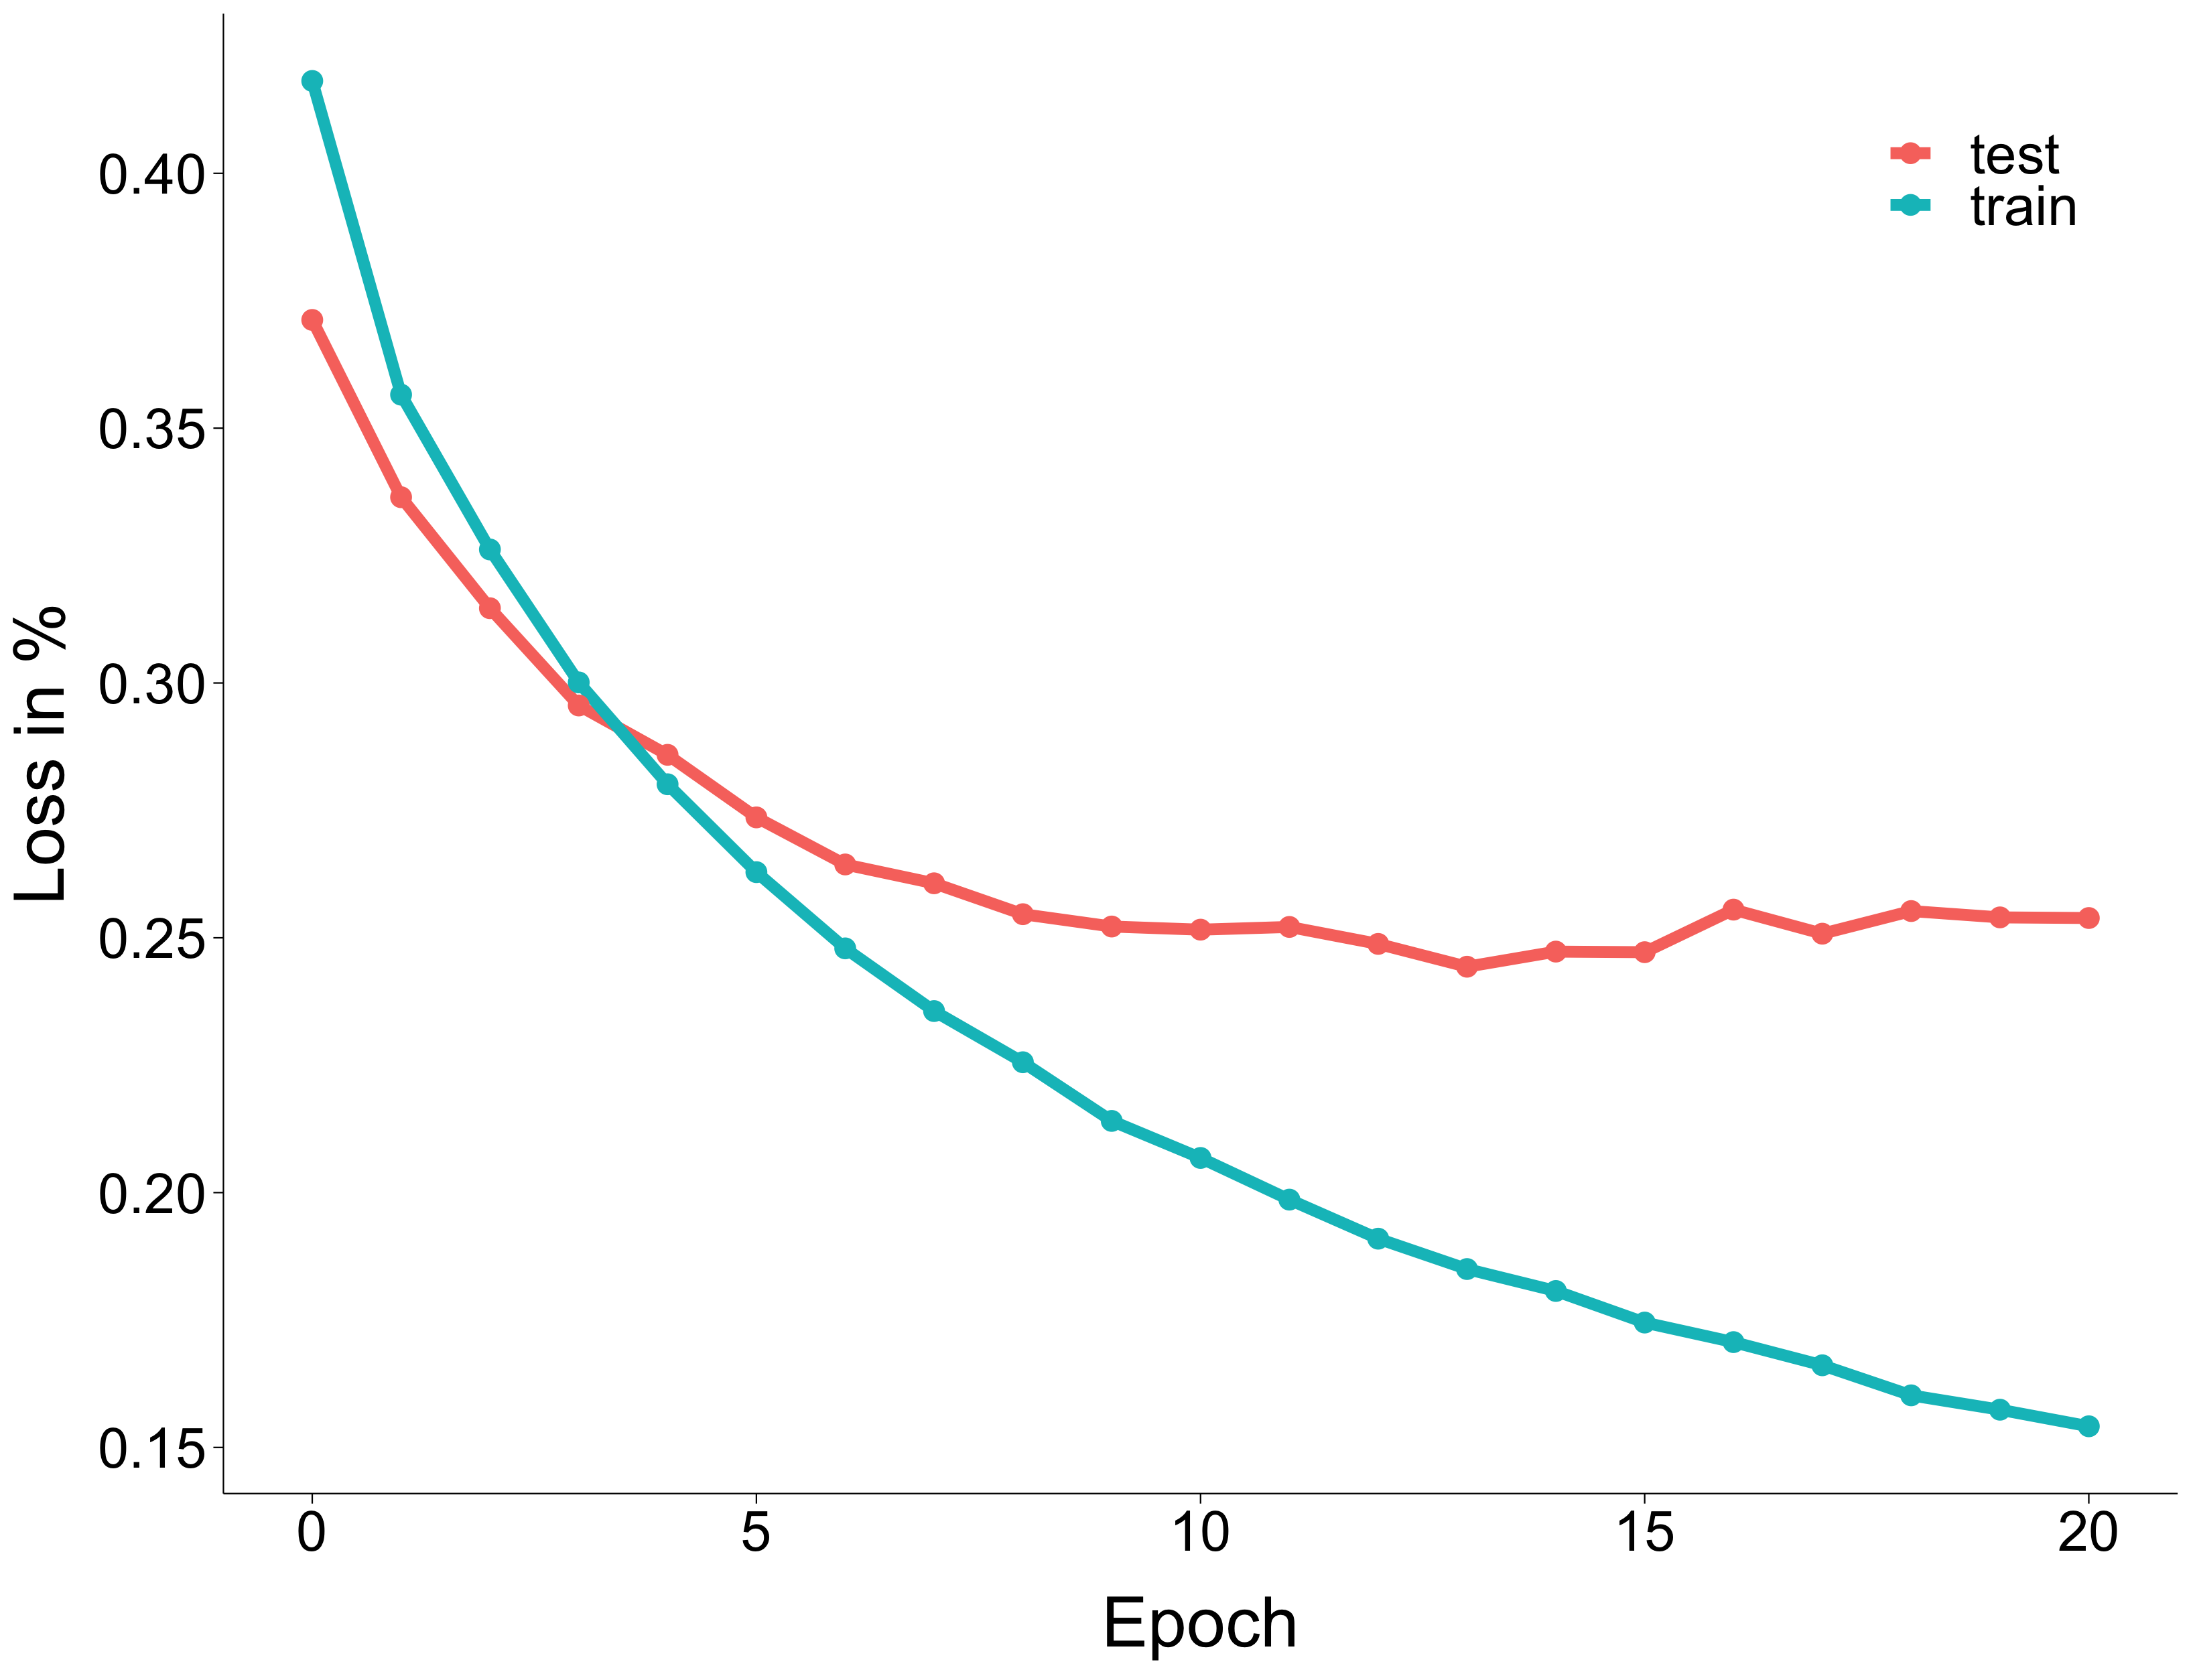
\includegraphics[width=0.6\textwidth]{figures/plot_model_losses}
%    \caption[Model losses on train and validation datasets.]{Model losses on train and validation datasets.}
%    \label{fig:plot-model-losses}
%\end{wrapfigure}

Accuracies (see Figure~\ref{fig:plot-model-accuracies}) were not rising significantly and losses (see Figure~\ref{fig:plot-model-losses}) for train and validation dataset departed after 21 epochs, so we stopped the training at this point.
We restored the weights from the best epoch (16) with an accuracy of 0.93 on the train and 0.90 on the test dataset.

\minisec{Predicting Story Character Genders}
The trained model was then used to predict the gender of each fictional character, their occurrences in the story and chapter were counted, and this information was then attached to the respective document.
In Section~\ref{sec:ner-token-classification}, we have already described how the story character names were extracted from the story texts.

To begin, we had to cleanse all the previously extracted story character names.
After some general clean-up operations, like removing special characters, numbers and whitespaces, we compared the names with the names from the training dataset.
If a match was found, the process was stopped immediately for that name, if not, we filtered words from the German \emph{DE-LIWC} dictionary~\citep{Meier2019LIWCDE-LIWC2015}.
For example, the name ``Glinda die Gute'' would become ``Glinda''.
Words were extracted from the \emph{LIWC 2015} poster in \emph{PDF} format using \emph{PyPDF2}\footnote{https://github.com/py-pdf/PyPDF2} and \emph{PDFMiner}\footnote{https://github.com/euske/pdfminer}.
Cleansed names with their cumulative occurrences were stored in the respective story document.

Given that iterating over each story in the corpus and predicting the genders of the story character names would have taken a significant amount of time, we split this process into several steps.

First, we extracted all story character names from the stories, removed any duplicates, and saved them to a separate \emph{CSV} file.
This newly created list was subsequently merged with the names from the training dataset and again duplicates were removed.
We then prepopulated additional information to the list, such as the gender and a probability value of 1.00 for all names from the training dataset.
This probability value was used to evaluate the confidence of the prediction, with 1.00 being the highest confidence and 0.00 being the lowest.

In the next step, this \emph{CSV} list was divided into 100 chunks with 2,800 stories each for the total 280,000 tagged stories.
Each chunk containing all the names from the 2,800 stories was then passed to the prediction model and the results with the predicted gender and probability were stored in a temporary data structure.
\begin{wrapfigure}{L}{0.65\textwidth}
    \centering
    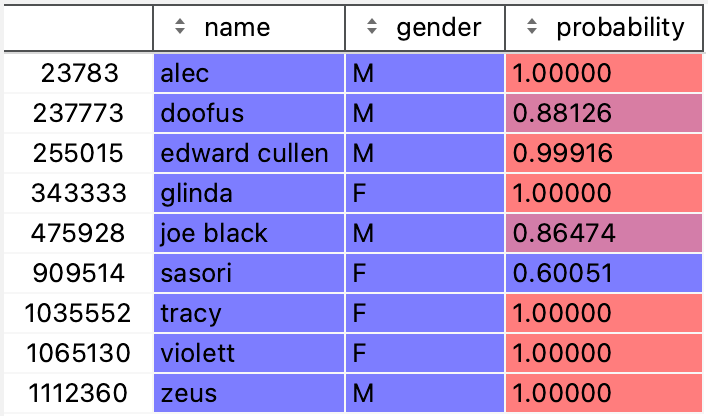
\includegraphics[width=0.55\textwidth]{figures/predicted_names_excerpt}
    \caption[Fragment of the \emph{CSV} list with the calculated gender of the names.]{Fragment of the \emph{CSV} list with the calculated gender of the names.}
    \label{fig:predicted-names-excerpt}
\end{wrapfigure}
After all chunks were processed, names with a low confidence of less than 0.80 and having at least one whitespace in the name were reprocessed.
The whitespaces were used to split the name into two parts, and the first part, a potential first name, was resent to the prediction model.
Finally, all prediction results were merged with the original list and saved in another \emph{CSV} file.
Figure~\ref{fig:predicted-names-excerpt} shows a fragment of this list to give an impression of what this looks like.

Utilizing this list, we iterated over all stories, comparing the names with the names from the prediction list.
Statistics showing the sum of all female, male, and indecisive names, along with their percentages and a female-to-male ratio, were then appended to the story document.
Whereas a ratio of 0.0 means that all decisive persons are female and 1.0 means that all are male, adapted from our one-hot coding for gender that we performed earlier for model training.
For example, a ratio of 0.7 means that the gender representation is rather male-dominated.
